% PROSZĘ KOMPILOWAĆ TEN DOKUMENT ZA POMOCĄ SILNIKA XELATEX
% W PRZECIWNYM RAZIE NALEŻY USUNĄĆ PAKIET fontspec ORAZ USTAWIENIA FONTU
% Z PLIKU styles/prez_wmini_pl.sty (PIERWSZE TRZY LINIJKI)
% W PRZYPADKU BRAKU FONTU Adagio Slab NALEŻY ZGŁOSIĆ SIĘ DO BIP PW O JEGO UDOSTĘPNIENIE,
% ZAŁADOWAĆ INNY KRÓJ CZCIONKI LUB ZAKOMENTOWAĆ/USUNĄĆ USTAWIENIA FONTU

\documentclass[aspectratio=169]{beamer}

\graphicspath{{images/}}

\usepackage{amssymb}
\usepackage{amsmath}
\usepackage{polski}
\usepackage[utf8]{inputenc}
\usepackage{hyperref}
\usepackage{blindtext}
\usepackage{multicol}
\usepackage{multirow}
\usepackage{wrapfig}
\usepackage{float}
\usepackage{enumitem}
\usepackage{xfrac}
\usepackage{caption}
\usepackage{subcaption}
\usepackage{booktabs}
\usepackage{wasysym}
\usepackage{xcolor}
\usepackage{pdfpages}
\usepackage{fontspec}
\usepackage{comment}
\usepackage{tocloft}
\usepackage{listings}
\usepackage{times}
\usepackage{amsmath}
\usepackage{bm}
\lstset{basicstyle=\ttfamily, columns=fullflexible}

\usepackage{caption, copyrightbox}
\captionsetup{justification=centering, labelfont=sc, labelsep=endash}

\usepackage{regexpatch}
\usepackage[os=mac]{menukeys}
\renewmenumacro{\keys}[+]{shadowedroundedkeys}
\renewmenumacro{\menu}[>]{angularmenus}
\xpatchcmd*{\SPACE}{2em}{1em}{}{}

\definecolor{quotationcolour}{HTML}{F0F0F0}
\definecolor{quotationmarkcolour}{HTML}{1F3F81}

% Double-line for start and end of epigraph.
\newcommand{\epiline}{\hrule \vskip -.2em \hrule}
% Massively humongous opening quotation mark.
\newcommand{\hugequote}{%
  \fontsize{42}{48}\selectfont \color{quotationmarkcolour} \textbf{``}
  \vskip -.5em
}

% Beautify quotations.
\newcommand{\epigraph}[2]{%
  \bigskip
  \begin{center}
  \colorbox{quotationcolour}{%
    \parbox{.80\textwidth}{%
    \epiline \vskip 1em {\hugequote} \vskip -.5em
    \parindent 2.2em
    #1\vspace{-.25cm}\begin{flushright}\textsc{#2}\end{flushright}
    \epiline
    }
  }
  \end{center}
  \bigskip
}

\setmainfont{Verdana}

\addtolength{\cftsecnumwidth}{5pt}
\addtolength{\cftsubsecnumwidth}{5pt}
\addtolength{\cftsubsubsecnumwidth}{5pt}
	
\usepackage{color, colortbl}
\definecolor{Gray}{gray}{0.9}

\definecolor{mGreen}{rgb}{0,0.6,0}
\definecolor{mGray}{rgb}{0.5,0.5,0.5}
\definecolor{mPurple}{rgb}{0.58,0,0.82}
\definecolor{backgroundColour}{rgb}{0.95,0.95,0.92}

\lstdefinestyle{CStyle}{
    backgroundcolor=\color{backgroundColour},   
    commentstyle=\color{mGreen},
    keywordstyle=\color{magenta},
    numberstyle=\tiny\color{mGray},
    stringstyle=\color{mPurple},
    basicstyle=\footnotesize,
    breakatwhitespace=false,         
    breaklines=true,                 
    captionpos=b,                    
    keepspaces=true,                 
    numbers=left,                    
    numbersep=5pt,                  
    showspaces=false,                
    showstringspaces=false,
    showtabs=false,                  
    tabsize=2,
    language=C
}

\usepackage[
backend=biber
,style=ieee
,sorting=none
]{biblatex}
\addbibresource{bibliografia.bib}
\DeclareNameAlias{author}{last-first}

\DeclareCiteCommand{\supercite}[\mkbibsuperscript]
  {\iffieldundef{prenote}
     {}
     {\BibliographyWarning{Ignoring prenote argument}}%
   \iffieldundef{postnote}
     {}
     {\BibliographyWarning{Ignoring postnote argument}}}
  {\usebibmacro{citeindex}%
   \bibopenbracket\usebibmacro{cite}\bibclosebracket}
  {\supercitedelim}
  {}
  
  \DeclareLabelalphaTemplate{
  \labelelement{
    \field[final]{shorthand}
    \field{label}
    \field[strwidth=3,strside=left,ifnames=1]{labelname}
    \field[strwidth=1,strside=left,final]{labelname}
    \field{labeltitle}
  }
  \labelelement{
    \field[strwidth=2,strside=right]{year}
  }
}

\renewcommand*{\figurename}{Rys.}

\usepackage{titlesec}
\titlelabel{\thetitle.\quad}

\usepackage{tikz}


\usetikzlibrary{matrix, ,backgrounds}
\usepackage{array}

\makeatletter
\tikzset{SWOT/.style={matrix of nodes,inner sep=0pt,row sep=0pt,column sep=0pt,
cells={nodes={anchor=center,inner sep=2pt}},
column 1/.style={nodes={rotate=90,minimum height=8mm}},
ampersand replacement=\&,
execute at end matrix={\begin{scope}[on background layer]
 \fill[black!10] (\tikz@fig@name.west|-\tikz@fig@name-2-2.north) rectangle 
  (\tikz@fig@name-\the\pgfmatrixcurrentrow-2.south west);
\end{scope}
\draw (\tikz@fig@name.west|-\tikz@fig@name-2-2.north) rectangle 
(\tikz@fig@name-\the\pgfmatrixcurrentrow-\the\pgfmatrixcurrentcolumn.south east)
 (\tikz@fig@name-1-2.north west) rectangle 
(\tikz@fig@name-\the\pgfmatrixcurrentrow-\the\pgfmatrixcurrentcolumn.south east)
(\tikz@fig@name-2-2.center|-\tikz@fig@name.north) --
 (\tikz@fig@name-2-2.center|-\tikz@fig@name.south)
foreach \XX in {2,...,\the\numexpr\pgfmatrixcurrentrow-1}
{(\tikz@fig@name-\XX-2.south-|\tikz@fig@name.west) --
(\tikz@fig@name-\XX-2.south-|\tikz@fig@name.east) };
}}}
\makeatother

\usepackage{tocloft}
\renewcommand\cftfigfont{\small}

\setlength{\parindent}{0pt}


\title{Adaptation of inertial navigation systems in parallel manipulator}
\subtitle{Master thesis presentation}
\author{Wojciech Gajda}
\date{January 23rd, 2023} % można tam wpisać datę jaką się chce lub zakomentować dla daty dzisiejszej



% ------------------ Początek prezentacji ------------------

\begin{document}
\sloppy

% Slajd tytułowy
{
\maketitleframe 
}

\begin{frame}
\frametitle{Agenda}
  \tableofcontents[  
    sectionstyle=show, 
    %hideallsubsections
    ]
\end{frame}

\section{Introduction}

\begin{frame}
	\frametitle{Motivation}
	\begin{columns}
		\begin{column}{0.5\textwidth}
			\begin{figure}
				\centering
				\uncover<2->{
					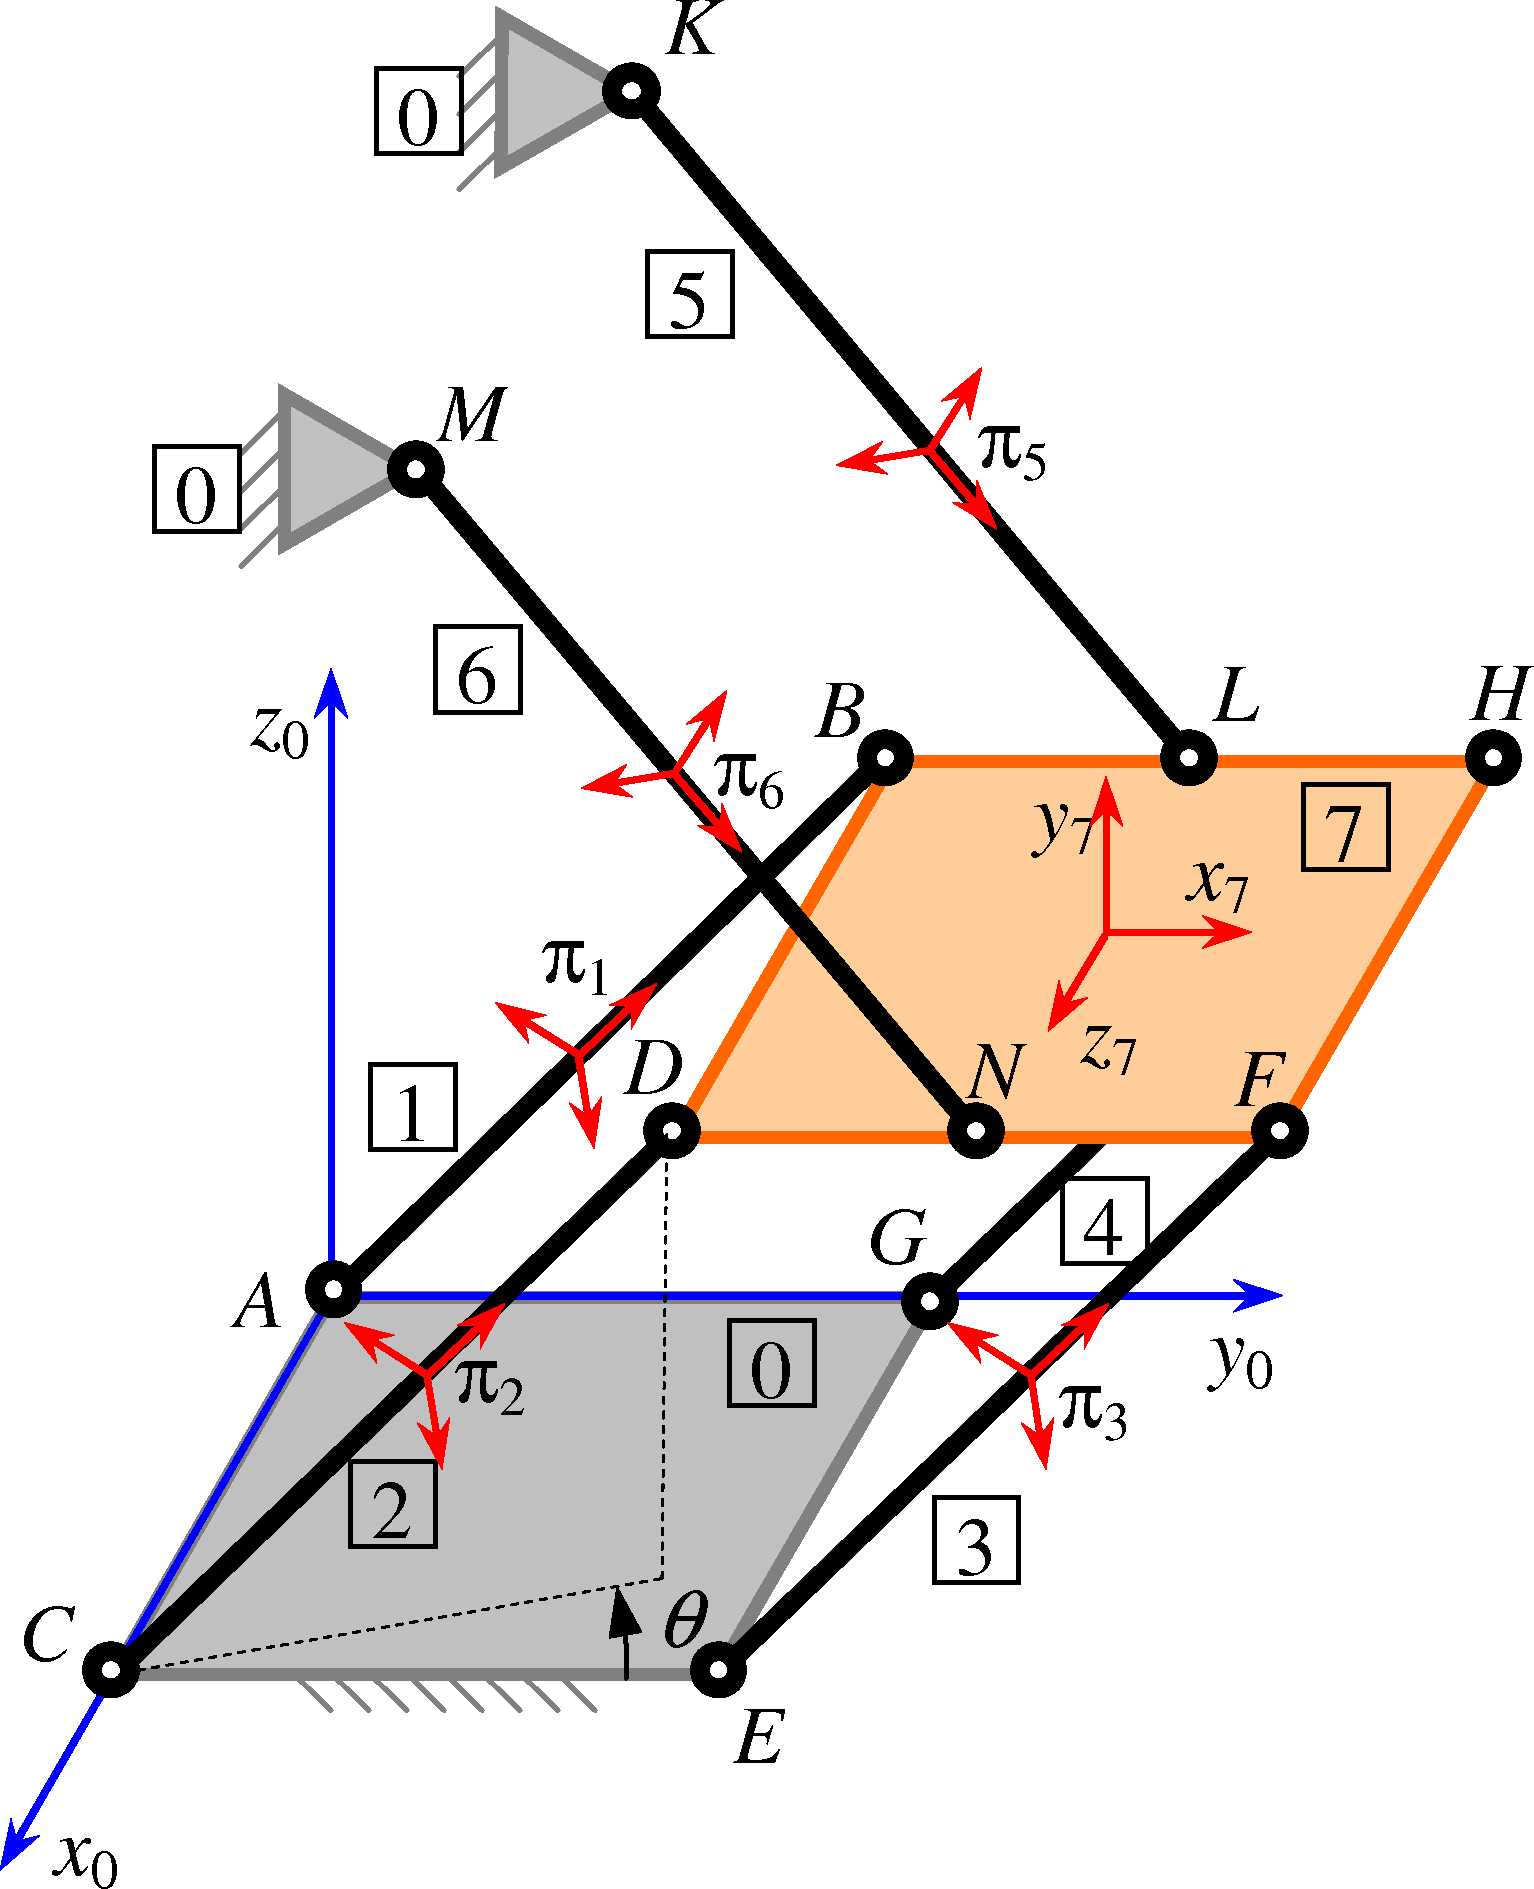
\includegraphics[height=0.75\textheight]{mbs_system.png}
					\caption{Multi-body system with 1 DOF}
				}
			\end{figure}
			\vspace{50pt}
		\end{column}
		\begin{column}{0.5\textwidth}
			\begin{figure}
				\centering
				\uncover<3->{
					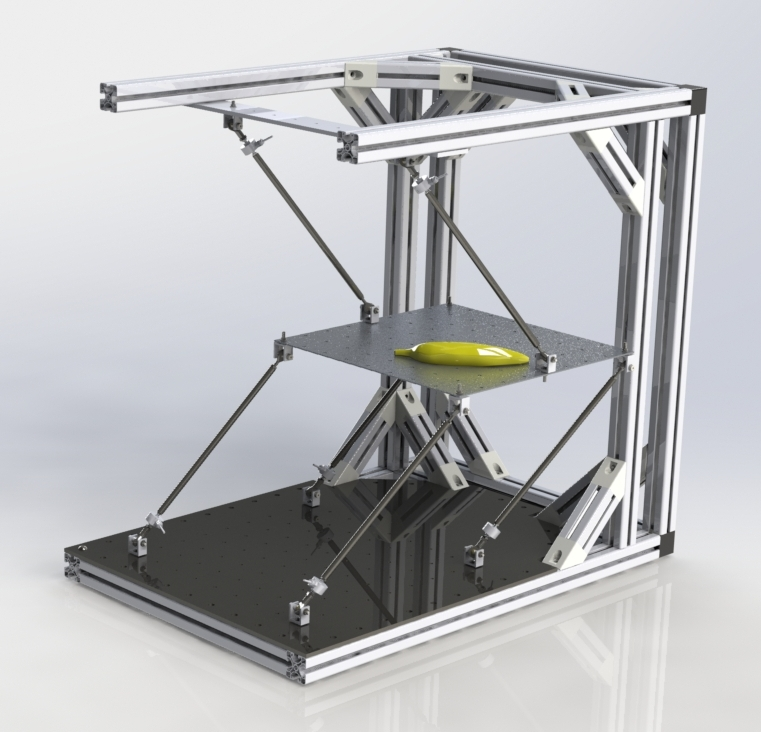
\includegraphics[height=0.75\textheight]{render.jpg}
					\caption{Render of MBS}
				}
			\end{figure}
			\vspace{50pt}
		\end{column}
	\end{columns}
\end{frame}


\begin{frame}
	\frametitle{Aim of the thesis}
	\begin{itemize}
		\setlength\itemsep{1em}
		\item<2-> Adaptation of inertial navigation system in robot positioning systems.
		\item<3-> Utilizing knowledge of design and constraints of the multi-body system.
		\item<4-> Review of sensor measurements filtration and fusion methods.
		\item<5-> Design of testing platform and prototype.
	\end{itemize}
\end{frame}

\section{The state of knowledge}

\begin{frame}
	\frametitle{Sensors}
	\begin{itemize}
		\item<2-> Accelerometer -- linear acceleration
		\item<3-> Gyroscope -- angular velocity
		\item<4-> \only<4>{Magnetometer -- magnetic field} \only<5->{\sout{Magnetometer -- magnetic field}}
		\item<6-> \only<6>{GNSS -- position \& velocity} \only<7->{\sout{GNSS -- position \& velocity}}
		\item<8-> \only<8>{Rangefinder} \only<9->{\sout{Rangefinder} Distance sensor}
	\end{itemize}
\end{frame}

\begin{frame}
	\frametitle{Sensor's error \& calibration}
	
	\uncover<2->{Error components:}
	\begin{itemize}
		\item<3-> Noise
		\item<4-> Bias
	\end{itemize}
	\centering
	\vspace{15pt}
	\uncover<5->{Sensors have finite resolution and sampling time.}
	\ \\
	\vspace{15pt}
	\uncover<6->{Bias is especially harmful, if measurements are integrated!}
\end{frame}

\begin{frame}
	\frametitle{Data filtration and fusion}
	% LPF HPF Smoothing filters Notch filters, adaptive filters, remove of outrunners
	
	
\end{frame}

\begin{frame}
	\frametitle{Extended Kalman Filter}
	\begin{itemize}
		\item<2-> The Extended Kalman Filter is an extension of the Kalman Filter for nonlinear systems.
		\item<3->  It is widely used in various fields, such as aviation, robotics, navigation, and control systems.
	\end{itemize}
	\vspace{10pt}
	\begin{center}
		\uncover<4->{
		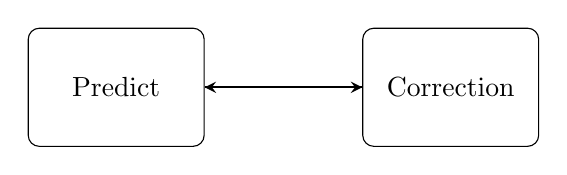
\begin{tikzpicture}[
			block/.style={rectangle, draw, text width=2cm, text centered, rounded corners, minimum height=1.5cm},
			arrow/.style={->, >=stealth, thick}
			]
			% Nodes
			\node (predict) [block] {Predict};
			\node (correct) [block, right=2cm of predict] {Correction};
			
			% Arrows
			\draw[arrow] (predict.east) -- ++(1.5cm,0) |- (correct.west) node[midway, above] {};
			\draw[arrow] (correct.west) -- ++(-1.5cm,0) |- (predict.east) node[midway, below] {};
		\end{tikzpicture}
		}
	\end{center}
\end{frame}

\begin{frame}
	\frametitle{EKF with constraint correction}
	\begin{itemize}
		\item<2-> Constraints based on multi-body system design
	\end{itemize}
	\vspace{10pt}
	\begin{center}
		\uncover<3->{
		\begin{tikzpicture}[
			block/.style={rectangle, draw, text width=2cm, text centered, rounded corners, minimum height=1.5cm},
			arrow/.style={->, >=stealth, thick},
			>=Stealth,
			]
			% Nodes
			\node (predict) [block] {Predict};
			\node (correct) [block, right=3cm of predict] {Correction};
			\node (constraints) [block, below left=0.5cm and 0.33cm of correct] {Constraints};
			
			% Arrows
			\draw[arrow] (predict.east)  |- (correct.west) node[midway, above] {};
			\draw[arrow] (correct.south)  |- (constraints.east) node[midway, left] {};
			\draw[arrow] (constraints.west) -- ++(-1.5cm,0) -| (predict.south) node[midway, below] {};
			
		\end{tikzpicture}
		}
	\end{center}
\end{frame}

\begin{frame}
	\frametitle{Simulation}
	%Synthetic-generated data.
	\begin{figure}
		\centering
		\includegraphics<2>[height=0.7\textheight]{no_corr.png}
		\includegraphics<3->[height=0.7\textheight]{corr.png}
		\caption{
			\only<2>{EKF without constraints}
			\only<3->{EKF with constraints}
		}
	\end{figure}
\end{frame}

\section{Summary}

\begin{frame}
	\frametitle{Summary}
\end{frame}

\begin{frame}
	\frametitle{Questions?}
	\begin{figure}
		\centering
		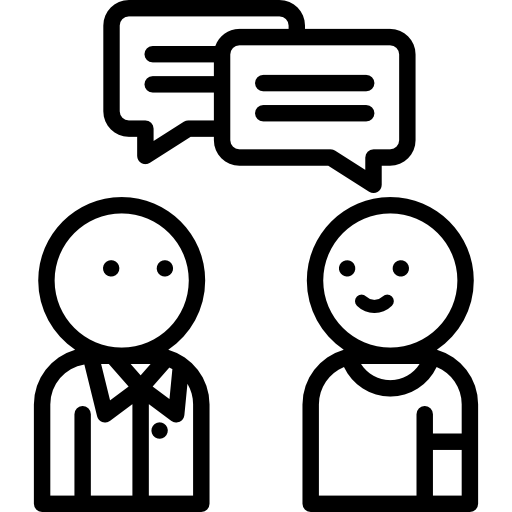
\includegraphics[width=0.7\textwidth]{questions.png}
	\end{figure}
\end{frame}

\begin{frame}
	  \begin{center}
	\Huge Thank you!
	\end{center}
\end{frame}

\end{document}